%!TEX root = ../dissertation.tex
\begin{savequote}[75mm]
This is some random quote to start off the chapter.
\qauthor{Firstname lastname}
\end{savequote}

\chapter{Analisi e progettazione}

\section{Metodo di lavoro}
Dopo un'attenta analisi delle esigenze di questo progetto, la metodologia che abbiamo deciso di utilizzare è Agile Kanban. Questa metodologia, ci ha permesso di avere un'alta flessibilità sui task da svolgere, una visione ampia del progetto e il focus su una singola attività alla volta.
La metodologia Kanban è stata scelta anche per affrontare l'esiguo numero del team, composto da sole 2 persone, con effettivamente solo una che lavorava a pieno regime su di esso.
Questo perché rendeva un'ottima visione dell'insieme delle attività da svolgere, in progresso e già svolte, oltre a non necessitare di ruoli predefiniti come nell'\gls{Agile Scrum}
\paragraph{Metodologia kanban}
Fa parte della famiglia delle metodologie agile, alla base vi è l'utilizzo di una lavagna nella quale vi è specificato uno stato per ogni colonna presente.
\begin{figure}[h!]
	\centering
	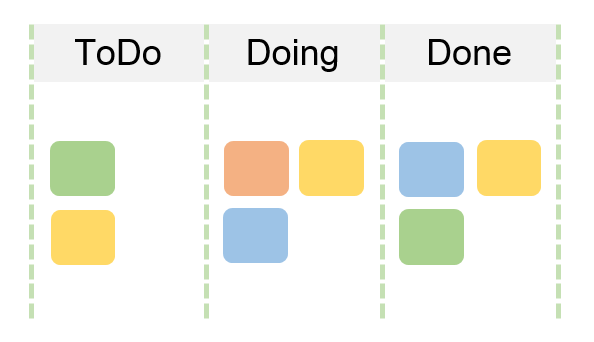
\includegraphics[scale=0.3]{figures/kanban-board}
	\caption[Short figure name.]{Esempio lavagna Kanban.
		\label{fig:logoGCP}}
\end{figure}	
Quello sopra riportato è uno degli esempi più semplici di lavagna Kanban, nella quale ogni task deve assumere tre stati per considerarsi completato "ToDo", "Doing" e "Done". Solitamente ogni componente del team ha la responsabilità di portare a completamente un solo task alla volta, così da evitare sovrapposizioni e confusione.
\section{Problemi affrontati}
\section{Pianificazione del lavoro}
Durante i colloqui svolti con il tutor aziendale, è stato redatto il piano di lavoro. Ciò ha portato la suddivisione dello stage in 8 parti, ognuna della durata di una settimana.
    \begin{itemize}
	\item[] \textbf{Prima Settimana (40 ore)}
	\begin{itemize}
		\item Incontro con persone coinvolte nel progetto per discutere i requisiti e le richieste
		relativamente al sistema da sviluppare;
		\item Verifica credenziali e strumenti di lavoro assegnati;
		\item Presa visione dell’infrastruttura esistente;
		\item Formazione sulle tecnologie adottate;
	\end{itemize}
	\item[] \textbf{Seconda Settimana (40 ore)} 
	\begin{itemize}
		\item Comprensione strumenti di storicizzazione;
		\item Analisi funzionamento filesystem distribuito;
		\item Produzione script Python per produzione dati simulati;
	\end{itemize}
	\item[] \textbf{Terza Settimana (40 ore)} 
	\begin{itemize}
		\item Caricamento dati su filesystem distribuito;
		\item Securizzazione accesso ai dati;
		\item Studio teorico approccio statistico al problema;
	\end{itemize}
	\item[] \textbf{Quarta Settimana (40 ore)} 
	\begin{itemize}
		\item Comprensione strumenti di processamento;
		\item Analisi funzionamento RDD;
		\item Implementazione processo batch con Python e Spark;        
	\end{itemize}
	\item[] \textbf{Quinta Settimana (40 ore)} 
	\begin{itemize}
		\item Analisi funzionamento Dataframe;
		\item Implementazione processo di elaborazione Spark;
		\item Ingegnerizzazione soluzione batch;
	\end{itemize}
	\item[] \textbf{Sesta Settimana (40 ore)} 
	\begin{itemize}
		\item Test prestazionale processo spark;
		\item Tuning prestazionale;
		\item Studio applicazione real-time;
	\end{itemize}
	\item[] \textbf{Settima Settimana (40 ore)} 
	\begin{itemize}
		\item Storicizzazione dati su storage persistente;
		\item Studio funzionamento Kafka;
		\item Implementazione processo real-time con Spark Streaming;
	\end{itemize}
	\item[] \textbf{Ottava Settimana - Conclusione (40 ore)} 
	\begin{itemize}
		\item Costruzione layer accesso al dato persistente;
		\item Ingegnerizzazione soluzione Spark Streaming;
		\item Integrazione storage persistente;
	\end{itemize}
\end{itemize}
possibili diagrammi
\section{Risultati}



